\documentclass{amsart}

\usepackage{amssymb}
\usepackage[margin=3cm]{geometry}
\usepackage{epigraph}
\usepackage{natbib}
\usepackage{xcolor}
\usepackage{hyperref}
\usepackage{tikz}

\begin{document}
\pagecolor{white}

\title{Red Queen's Sync Protocol for Ethereum}
\author{Andrew Ashikhmin \& Alexey Akhunov}
\date{March 2019}

\begin{abstract}
TODO: abstract.
\end{abstract}

\maketitle

\epigraph{
    "A slow sort of country!" said the Queen.
    "Now, here, you see, it takes all the running you can do, to keep in the same place.
    If you want to get somewhere else, you must run at least twice as fast as that!"
    }{Lewis Carroll, Through the Looking-Glass and What Alice Found There}

\section{Introduction}

In Red Queen's Synchronisation Protocol for Ethereum 1x seeders reply with data as of their most recent block.
That results in an inconsistent trie on the leecher initially ("phase 1"), which we patch later ("phase 2").
The idea is similar to that of Leaf Sync (\cite{leaf_sync}).

TODO: mention the sync failure problem \cite{akhunov_1x_workshop_part1} and the needs of light clients like Mustekala.
Inspirations like BitTorrent, Parity's warp sync,
\href{https://notes.ethereum.org/eXnqtO_vQquzrFDPHjuaFQ}{Firehose Sync},
\href{https://github.com/ethereum/wiki/wiki/Light-client-protocol}{Light Client Protocol}.

N.B. Snapshot synchronisation rather than from the Genesis block.


% TODO https://ethereum-magicians.org/t/forming-a-ring-eth-v64-wire-protocol-ring/2857/4

\section{Notation}

We mostly follow the conventions and notations of the Yellow Paper (\cite{yellow_paper}),
for instance, $\mathbb{Y}$ denotes the set of nibble sequences.
We use the letter $\pi$ for prefixes of state or storage trie keys $\mathbf{k} \in \mathbb{B}_{32}$,
\begin{equation}
    \pi \in \mathbb{Y} \; \land \; ||\pi|| \leq 64
\end{equation}
A key matches a prefix if and only if all their first nibbles are the same,
\begin{equation}
    \texttt{MATCH}(\mathbf{k}, \pi) \equiv \forall_{i < ||\pi||}: \mathbf{k}'[i] = \pi[i]
\end{equation}
($\mathbf{k}'$ is a sequence of nibbles, while $\mathbf{k}$ is a sequence of bytes.)

\section{Protocol Specification}

We propose the following 3 request/reply operative pairs.

\textbf{GetStorageSizes} [+0x20, reqID: $\mathbb{N}$, blockAtLeast: $\mathbb{N}$,
[account$^0$: $\mathbb{B}_{32}$, account$^1$: $\mathbb{B}_{32}$, ...]]
Request storage trie sizes as of block \#$\texttt{blockAtLeast}$ or newer.
Hashes of accounts addresses are used as keys.

\textbf{StorageSizes} [+0x21, reqID: $\mathbb{N}$, blockNumber: $\mathbb{N}$, blockHash: $\mathbb{B}_{32}$,
[numLeaves$^0$: $\mathbb{N} | \varnothing$, numLeaves$^1$: $\mathbb{N} | \varnothing$, ...]]
Reply to $\texttt{GetStorageSizes}$.
Returns storage trie sizes as of block \#$\texttt{blockNumber} \geq \texttt{blockAtLeast}$.
The elements returned must strictly match the accounts requested.
The peer may return the empty list $\varnothing$ instead of the number of leaves for accounts it does not have enough information about.

\textbf{GetNodeData2} [+0x22, reqID: $\mathbb{N}$, blockAtLeast: $\mathbb{N}$,
[account$^0$: $\mathbb{B}_{32} | \varnothing$, prefix$^0_0$: $\mathbb{Y}$, prefix$^0_1$: $\mathbb{Y}$, ...],
[account$^1$: $\mathbb{B}_{32} | \varnothing$, prefix$^1_0$: $\mathbb{Y}$, prefix$^1_1$: $\mathbb{Y}$, ...],
...]
Request state or storage trie nodes as of block \#$\texttt{blockAtLeast}$ or newer.
The empty list $\varnothing$ instead of the account hash signifies the state (rather than storage) trie.
Note that this operative is similar to $\texttt{GetNodeData}$ from Ethereum Wire Protocol PV63,
but it uses prefixes rather than hashes as node keys\footnote{For
a justification see Péter Szilágyi's
\href{https://ethereum-magicians.org/t/forming-a-ring-eth-v64-wire-protocol-ring/2857/10}{comment}
at ETH v64 Wire Protocol Ring.}.
TODO: prefix--node correspondence is trivial for branch nodes, not so much for leaf or extension nodes.
TODO: prefix encoding consistent with the Yellow Paper.

\textbf{NodeData2} [+0x23, reqID: $\mathbb{N}$, blockNumber: $\mathbb{N}$, blockHash: $\mathbb{B}_{32}$,
[node$^0_0$: $\mathbb{B}$, node$^0_1$: $\mathbb{B}$, ...],
[node$^1_0$: $\mathbb{B}$, node$^1_1$: $\mathbb{B}$, ...],
...]
Reply to $\texttt{GetNodeData2}$.
Returns trie nodes as of block \#$\texttt{blockNumber} \geq \texttt{blockAtLeast}$.
The nodes returned must strictly match the prefixes requested.
The empty list $\varnothing$ returned instead of a node means that the peer does not have enough information about the node requested.

\textbf{GetSubtries} [+0x24, reqID: $\mathbb{N}$, blockAtLeast: $\mathbb{N}$,

\quad [account$^0$: $\mathbb{B}_{32} | \varnothing$,

\qquad [prefix$^0_0$: $\mathbb{Y}$, fromLevel$^0_0$: $\mathbb{N}$],

\qquad [prefix$^0_1$: $\mathbb{Y}$, fromLevel$^0_1$: $\mathbb{N}$],

\qquad ...

\quad ],

\quad [account$^1$: $\mathbb{B}_{32} | \varnothing$,

\qquad [prefix$^1_0$: $\mathbb{Y}$, fromLevel$^1_0$: $\mathbb{N}$],

\qquad [prefix$^1_1$: $\mathbb{Y}$, fromLevel$^1_1$: $\mathbb{N}$],

\qquad ...

\quad ],

\quad ...

] Request state or storage subtrie leaves along with proof nodes as of block \#$\texttt{blockAtLeast}$ or newer.
The empty list $\varnothing$ instead of the account hash signifies state rather than storage trie.
$\texttt{fromLevel}$ specifies the number of upper nodes to be excluded from the proof in case the chain has not moved ahead (reply block is not newer).

\textbf{Subtries} [+0x25, reqID: $\mathbb{N}$, blockNumber: $\mathbb{N}$, blockHash: $\mathbb{B}_{32}$,

\quad [

\qquad [[node$^0_{00}$: $\mathbb{B}$, node$^0_{01}$: $\mathbb{B}$, ...], tooManyLeaves$^0_0$, [key$^0_{00}$: $\mathbb{B}_{32}$, val$^0_{00}$: $\mathbb{B}$, key$^0_{01}$: $\mathbb{B}_{32}$, val$^0_{01}$: $\mathbb{B}$, ...]$_{opt}$],

\qquad [[node$^0_{10}$: $\mathbb{B}$, node$^0_{11}$: $\mathbb{B}$, ...], tooManyLeaves$^0_1$, [key$^0_{10}$: $\mathbb{B}_{32}$, val$^0_{10}$: $\mathbb{B}$, key$^0_{11}$: $\mathbb{B}_{32}$, val$^0_{11}$: $\mathbb{B}$, ...]$_{opt}$],

\qquad ...

\quad ],

\quad [

\qquad [[node$^1_{00}$: $\mathbb{B}$, node$^1_{01}$: $\mathbb{B}$, ...], tooManyLeaves$^1_0$, [key$^1_{00}$: $\mathbb{B}_{32}$, val$^1_{00}$: $\mathbb{B}$, key$^1_{01}$: $\mathbb{B}_{32}$, val$^1_{01}$: $\mathbb{B}$, ...]$_{opt}$],

\qquad [[node$^1_{10}$: $\mathbb{B}$, node$^1_{11}$: $\mathbb{B}$, ...], tooManyLeaves$^1_1$, [key$^1_{10}$: $\mathbb{B}_{32}$, val$^1_{10}$: $\mathbb{B}$, key$^1_{11}$: $\mathbb{B}_{32}$, val$^1_{11}$: $\mathbb{B}$, ...]$_{opt}$],

\qquad ...

\quad ],

\quad ...

] Reply to $\texttt{GetSubtries}$.
Returns subtrie leaves with proofs as of block \#$\texttt{blockNumber} \geq \texttt{blockAtLeast}$.
The subtries returned must strictly match the prefixes requested.
If the peer does not have information regarding a particular subtrie, it should return the empty list $\varnothing$ (e.g. []) rather than [nodes, tooManyLeaves, leaves] for it.
The nodes returned are the upper nodes of the trie down to the subtrie root, so that it is possible to verify that the leaves do belong to the Merkle Patricia trie in question.
The first $\texttt{fromLevel}$ upper nodes must be skipped if and only if $\texttt{blockNumber} = \texttt{blockAtLeast}$.
(If $\texttt{fromLevel} = 0$, then the nodes must start with the root node.)
$\texttt{tooManyLeaves}$ is a boolean flag ($0=false$, $1=true$) indicating that the subtrie requested contains too many leaves.
TODO: how many is too many?
The leaves are represented as the list of their keys\footnote{It
is feasible to return suffixes rather than full keys given that prefixes are known, but we deem the performance gain to be insignificant.}
and values.
The peer may only return either all leaves of the subtrie or nothing.
In the case of $\texttt{tooManyLeaves}$ the leaves should not be returned\footnote{In
that case the peer must not return an empty list as that would imply that no leaves match the given prefix.}.
Proof nodes must be sent in any case;
they give us a means to detect faulty or malicious peers.
Note that state trie replies do not inline storage tries, unlike Leaf Sync.\\

TODO: is block number OK given chain reorgs?

\section{Suggested Sync Algorithm}

Here we suggest a possible algorithm for full state and storage snapshot synchronisation using the protocol specified above;
light clients are out of scope.
We describe a modus operandi where the seeder replies with its most recent data,
and the leecher has to handle trie data coming from different blocks.
We suggest to perform synchronisation in two stages:
during phase~1 the leecher obtains leaf data (with the necessary proof nodes) as of any reasonable block height,
while during phase~2 it patches up the trie in order to catch up to the most recent block\footnote{The
Red Queen's race is a nice metaphor for phase 2.}.
The idea was proposed in \cite{leaf_sync}.

Let us focus on the state trie for the moment; we shall come back to storage sync later.
For phase 1 we suggest sending $\texttt{GetSubtries}$ requests with a single prefix per request, ditto for phase 2.
All requested prefixes are of size $d_1$ during phase 1 and of $d_2$ during phase 2, $d_2 \geq d_1$.
We elaborate on the values of $d_1$ and $d_2$ later.
The leecher gradually builds the first upper $d_2$ levels of the Merkle Patricia trie\footnote{$d_2$
is small enough so that we can reasonably assume that (almost) all nodes in question are branch nodes;
see \cite{akhunov_1x_workshop_part2}.}.
(The full trie can be constructed if so desired, but only the upper $d_2$ levels are necessary for our algorithm.)
Populated nodes are marked with the block number as of they are valid.
The algorithm preserves the following invariant: parent's block is always no older than child's block.

During phase 1 the leecher requests each possible prefix of size $d_1$ exactly once
(barring network failures and faulty peers).
When sending a request,
the leecher sets its $\texttt{blockAtLeast}$ to the block of the root of the current (partially populated) trie,
$\texttt{fromLevel}$ to the number of populated nodes down the path/prefix that are of the same block as the root.
Having received a reply, the leecher verifies its proof.
If the proof is valid, the leecher writes received leaves to the database and updates the nodes along the prefix/path.
By the end of phase 1, the leecher will have all accounts populated, albeit inconsistently.

\begin{figure}
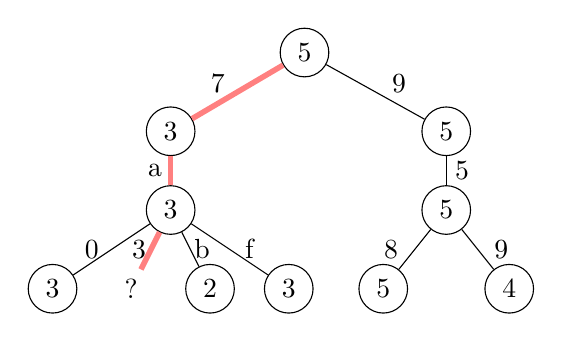
\begin{tikzpicture} [scale=1, auto=left]
\tikzstyle{selected edge} = [draw,line width=2pt,-,red!50]

  \node[circle,draw] (n)       at (4.2,4) {5};
  \node[circle,draw] (n7)     at (2.5,3) {3};
  \node[circle,draw] (n9)     at (6,3)    {5};
  \node[circle,draw] (n7a)   at (2.5,2) {3};
  \node[circle,draw] (n95)   at (6,2)    {5};
  \node[circle,draw] (n7a0) at (1,1)    {3};
  \node(n7a3) at (2,1)    {?};
  \node[circle,draw] (n7ab) at (3,1)    {2};
  \node[circle,draw] (n7af)  at (4,1)    {3};
  \node[circle,draw] (n958) at (5.2,1) {5};
  \node[circle,draw] (n959) at (6.8,1) {4};

  \draw[selected edge] (n) -- (n7);
  \draw (n) -- (n9);
  \draw[selected edge] (n7) -- (n7a);
  \draw (n9) -- (n95);
  \draw (n7a) -- (n7a0);
  \draw[selected edge] (n7a) -- (n7a3);
  \draw (n7a) -- (n7ab);
  \draw (n7a) -- (n7af);
  \draw (n95) -- (n958);
  \draw (n95) -- (n959);
  
  \node at (1.5, 1.5) {0};
  \node at (2.1, 1.5) {3};
  \node at (2.9, 1.5) {b};
  \node at (3.5, 1.5) {f};
  
  \node at (5.3, 1.5) {8};
  \node at (6.7, 1.5) {9};
  
  \node at (2.3, 2.5) {a};
  \node at (6.2, 2.5) {5};
  
  \node at (3.1, 3.6) {7};
  \node at (5.4, 3.6) {9};
\end{tikzpicture}
\setlength{\unitlength}{2cm}
\begin{picture}(1,1)
\put(0.2,0.9){\line(1,0){0.5}}
\put(0.2,1.1){\line(1,0){0.5}}
\put(0.8,1){\line(-1,1){0.2}}
\put(0.8,1){\line(-1,-1){0.2}}
\end{picture}
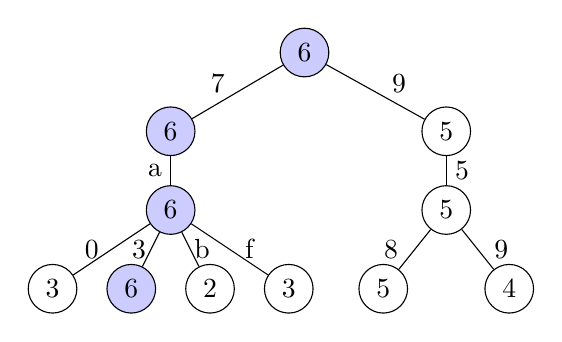
\begin{tikzpicture} [scale=1,auto=left]
  
  \node[circle,draw,fill=blue!20] (n)       at (4.2,4) {6};
  \node[circle,draw,fill=blue!20] (n7)     at (2.5,3) {6};
  \node[circle,draw] (n9)     at (6,3)    {5};
  \node[circle,draw,fill=blue!20] (n7a)   at (2.5,2) {6};
  \node[circle,draw] (n95)   at (6,2)    {5};
  \node[circle,draw] (n7a0) at (1,1)    {3};
  \node[circle,draw,fill=blue!20] (n7a3) at (2,1)    {6};
  \node[circle,draw] (n7ab) at (3,1)    {2};
  \node[circle,draw] (n7af)  at (4,1)    {3};
  \node[circle,draw] (n958) at (5.2,1) {5};
  \node[circle,draw] (n959) at (6.8,1) {4};

  \draw (n) -- (n7);
  \draw (n) -- (n9);
  \draw (n7) -- (n7a);
  \draw (n9) -- (n95);
  \draw (n7a) -- (n7a0);
  \draw (n7a) -- (n7a3);
  \draw (n7a) -- (n7ab);
  \draw (n7a) -- (n7af);
  \draw (n95) -- (n958);
  \draw (n95) -- (n959);
  
  \node at (1.5, 1.5) {0};
  \node at (2.1, 1.5) {3};
  \node at (2.9, 1.5) {b};
  \node at (3.5, 1.5) {f};
  
  \node at (5.3, 1.5) {8};
  \node at (6.7, 1.5) {9};
  
  \node at (2.3, 2.5) {a};
  \node at (6.2, 2.5) {5};
  
  \node at (3.1, 3.6) {7};
  \node at (5.4, 3.6) {9};
\end{tikzpicture}
\caption{Illustration of phase 1 sync. Nodes are labelled with block numbers, and edges are labelled with nibbles.}
\label{fig:phase1_example}
\end{figure}

Figure~\ref{fig:phase1_example} shows an example of a phase 1 step with $d_1 = 3$ and $d_2 = 4$.
Say the leecher is interested in prefix $<$7a3$>$.
The trie on the left represents leecher's state before sending a request.
Root's block is 5, so it sets $\texttt{blockAtLeast} = 5$.
The leecher sets $\texttt{fromLevel}$ to 1 since there is no need to re-send the root as part of the proof.
It cannot set $\texttt{fromLevel}$ higher as the other nodes along the path are older than the root and thus have to be refreshed.
Suppose that the seeder replies with data as of a newer block \#6.
Since the block has changed, the seeder ignores $\texttt{fromLevel}$ and sends full proof.
The leecher saves received leaves to its database and updates the nodes  ($<>$, $<$7$>$, $<$7a$>$, $<$7a3$>$).
The result is displayed on the right of Figure~\ref{fig:phase1_example}.

At the beginning of phase 2, the leecher updates the trie in order to figure out which subtries have to be refreshed.
For that, it uses the $\texttt{GetNodeData2}$ operative.
The leecher refreshes the trie level by level, starting from the root (level 0) and descending to the level $d_2 - 1$.
Nodes at the same level may be requested in batch.
Having refreshed nodes for a level, it knows which child nodes one level below have to be refreshed since the leecher can compare their hashes it currently holds with received fresh data.
Therefore, only the nodes that have actually changed need to be requested.
The leecher might have to restart the node refresh process from the root if new blocks are mined in between;
however, provided a certain network bandwidth, the process converges.
We analyse convergence conditions in the next section.

When all trie levels from the root down to the level $d_2 - 1$ are up to date,
the leecher knows which nibbles at that last level have changed since phase 1.
It refreshes the leaves corresponding to such nibbles using $\texttt{GetSubtrie}$ requests. 
That concludes the algorithm for state trie synchronisation.

The algorithm for storage sync is similar for large storage tries.
Its parameters $d_1$ and $d_2$ are optimised based on the storage size as described in the next section.
Small storage tries can be obtained in bulk requesting the empty prefix (meaning the entire trie) for a number of them in one go.
$\texttt{GetStorageSizes}$ provides a means of finding out storage sizes.

\section{Performance Analysis}

In this analysis, we assume that all tries are well balanced.
We also assume that all top nodes up to a certain trie level $i$ are branch nodes, not leaf nor extension nodes.
This is a reasonable assumption if $i$ is not too big---see~\cite{akhunov_1x_workshop_part2}.
And we simplify the byte size function of the replies\footnote{Total
request size is much smaller than total reply size, so we ignore requests as well.},
ignoring overheads caused by auxilary data such as $\texttt{reqID}$,
RLP encoding, and the network layer.
%TODO: internal notation consistency + cross-check against the Yellow Paper
Let us introduce some notation:

$s_n$ -- the average node size in bytes,
equal essentially to the size of a branch node as most nodes transferred will be branch nodes.
530 bytes is a good estimate.

$s_l$ -- the average leaf size in bytes, counting both key and value.
For the state trie it is the average account size plus the size of its hash key,
resulting in about 115 bytes.
TODO: storage trie.

$t$ -- total number of leaves in a trie.
For the state trie it is the number of accounts,
which is about $53 \cdot 10^6$ as of February 2019---see \cite{akhunov_1x_workshop_part2}.

$||R_n||$ -- the number of nodes in a reply $R$.

$||R_l||$ -- the number of leaves in a reply $R$ (only relevant for $\texttt{Subtrie}$ replies).

We use the following simplified formula for the byte size of a reply $R$
\begin{equation}
    S(R) = ||R_n|| s_n + ||R_l|| s_l
\end{equation}

The overhead of the sync algorithm during phase 1, compared with Parity's warp sync, is in the proof nodes sent alongside the leaf data.
Their number is, roughly speaking, equal to the size of a Merkle Patricia trie of depth $d_1$, times the number of block changes during phase 1.
So, to reduce the overhead, we want $d_1$ to be as low as possible.
On the other hand, small $d_1$ implies a large number of leaves per reply, which can be brittle or inefficient.
Thus we set $d_1$ to the smallest value possible such that the replies are, on average, no larger than a certain size (say 32 KB).
We denote that maximum size as $m$.
During phase 1 a $\texttt{Subtrie}$ reply contains at most $d_1$ nodes
and its average number of leaves is $\frac{t}{16^{d_1}}$,
which gives us
\begin{equation}
    d_1 s_n + \frac{t}{16^{d_1}} s_l \leq m
\end{equation}
Fot the state trie the limit of 32 KB yields $d_1 = 5$.

TODO: revisit the reasoning (and $d_2$ in the code) after subtrieHash removal.
Now let us find the maximum size $d$ of the request prefix $\pi$ that makes sense to use when we are catching up (phase 2 of the sync).
Let assume that only one leaf that matches $\pi$ has changed.
(If we know that there are no changes, there is no need for a sync request.)
That is a reasonable assumption if we are not too many blocks behind, there are not that many changes per block, and $d$ is sufficiently large.
(For instance, if we are 100 blocks behind, and there are 500 leaf changes per block, then $d \geq 4$ will suffice.)
Consider two options: request the prefix $\pi$ or send requests with prefixes $\pi \cdot 0, ..., \pi \cdot 15$ of size $d+1$
(not necessarily all 16 of them).
In the first case, we receive a reply of the size, on average,
\begin{equation}
    S = o + ||R_b|| b + \frac{t}{16^d} l
\end{equation}
For the second case, we need to send at most two requests,
as the first reply gives us the information to identify which nibble has changed.
(With the probability $\frac{1}{16}$ the second request is not necessary.)
The combined size of those 1 or 2 replies, on average, is
\begin{equation}
    S' = \left( 1 + \frac{15}{16} \right) o + (||R_b|| + 1) b + \frac{t}{16^{d+1}} l
\end{equation}
It does not make sense to prefer requests with longer prefixes if $S \leq S'$.
Solving this inequality, we obtain
\begin{equation}
    16^d (16b + 15o) \geq 15tl
\end{equation}
Hence we can set the sync algorithm parameter $d_2$ as
\begin{equation}
d_2 = \left\lceil \log_{16} \frac{15tl} {16b + 15o} \right\rceil
\end{equation}

TODO: convergence analysis.

\section{Conclusion}

TODO: conclusion.

\bibliographystyle{plainnat}
\bibliography{biblio}

% TODO reference Firehose Sync, Light client protocol, etc.

\end{document}
